\documentclass[mathserif,18pt,xcolor=table]{beamer}

% Load Beamer Style Theme
% TAMU Based
\usepackage{tamu_beamer}
% \usepackage[skip=0pt]{caption}

% \preto\subequations{\ifhmode\unskip\fi}
% \AtBeginEnvironment{subequations}{\ifhmode\unskip\fi}
% \AtBeginEnvironment{equation}{\ifhmode\unskip\fi}
\makeatletter
\g@addto@macro\normalsize{%
\setlength\abovedisplayskip{0pt}
\setlength\belowdisplayskip{0pt}
\setlength\abovedisplayshortskip{0pt}
\setlength\belowdisplayshortskip{0pt}
}
\makeatother


% Specifiy the location of images to be used
\graphicspath{{figures/}}

% ------------------------------------------------------------
% ------------------------------------------------------------
% ------------------------------------------------------------
% ----------------TITLE PAGE----------------------------------
% ------------------------------------------------------------
% ------------------------------------------------------------
% ------------------------------------------------------------
% Document Title Page
\title{Surface wave supporting structures in the terahertz and optical frequency domains}
% \subtitle{Preliminary Exam}
\author[Hasan Tahir Abbas]{Hasan Tahir Abbas\\~\\{\small {Supervised by: Dr. Robert D. Nevels}}}
\institute{Department of Electrical  \& Computer Engineering\\ \mbox{} \\ \pgfuseimage{tamuecenbig}}
\date[Summer 2017]{\today}
% ------------------------------------------------------------
% ------------------------------------------------------------
% ------------------------------------------------------------
% ------------------------------------------------------------
% ------------------------------------------------------------
% ------------------------------------------------------------
% ------------------------------------------------------------
% ------------------------------------------------------------
% ------------------------------------------------------------
% ------------------------------------------------------------
% ------------------------------------------------------------
% ------------------------------------------------------------
% ------------------------------------------------------------
% ------------------------------------------------------------
\begin{document}

% Reduce space around equations and subequations
\preto\subequations{\ifhmode\unskip\fi}
\AtBeginEnvironment{subequations}{\ifhmode\unskip\fi}
\AtBeginEnvironment{equation}{\ifhmode\unskip\fi}

% Draw Boxes in the footer with pertinent info
\tikzstyle{block} = [rectangle, draw, rounded corners, shade, top color=white, text width=5em,
bottom color=blue!50!black!20, draw=blue!40!black!60, very thick, text centered, minimum height=4em]
\tikzstyle{line} = [draw, -latex']
\tikzstyle{cloud} = [draw, ellipse,top color=white, bottom color=red!20, node distance=2cm, minimum height=2em]

% Tick Style
\beamertemplateballitem
% \beamertemplatetransparentcoveredhigh

\frame{\titlepage}


% Add TAMU logo on each slide in the north-east side
% Shifted to be right at the edge
%
% NOTE: Will have to compile twice
%
\addtobeamertemplate{frametitle}{}{%
\begin{tikzpicture}[remember picture,overlay]
\node[anchor=north east,yshift=7pt,xshift=2pt] at (current page.north east) {
\includegraphics[height=.7cm]{ecen}};
\end{tikzpicture}}
% ------------------------------------------------------------
% ------------------------------------------------------------
% ------------------------------------------------------------
% ------------------------------------------------------------
% ------------------------------------------------------------
% ------------------------------------------------------------
% ------------------------------------------------------------
% ------------------------------------------------------------
% ------------------------------------------------------------
% ------------------------------------------------------------
% ------------------------------------------------------------
% ------------------------------------------------------------
% ------------------------------------------------------------
% ------------------------------------------------------------
\section{Outline}
\begin{frame}
  \frametitle{Outline}
  \framesubtitle{Dissertation Defense}
  \begin{itemize}
    \item Plasmonics Overview
    \item Background
    \item Theory and Methods
    \begin{itemize}
      \item[-]{Dispersion Relation}
      \item[-]{Surface Integral equation}
    \end{itemize}
    \item Results
    \item Proposed Work
  \end{itemize}
\end{frame}
% ------------------------------------------------------------
% ------------------------------------------------------------
% ------------------------------------------------------------
% ------------------------------------------------------------
% ------------------------------------------------------------
% ------------------------------------------------------------
% ------------------------------------------------------------
% ------------------------------------------------------------
% ------------------------------------------------------------
% ------------------------------------------------------------
% ------------------------------------------------------------
% ------------------------------------------------------------
% ------------------------------------------------------------
% ------------------------------------------------------------
\section{Overview}
% ------------------------------------------------------------
% ------------------------------------------------------------
\begin{frame}
  \frametitle{Plasmonics Overview}
  % ----------------------------------------------------------
  \begin{columns} % align columns
    \begin{column}{.5\textwidth}
      \begin{itemize}
        \item Interaction of electromagnetic (EM) waves with surfaces
        \item Surface plasmon waves
        \item Two-dimensional materials
        \item Miniaturization of circuit and antenna devices
        \item Terahertz gap
        \item Poor energy efficiencies
      \end{itemize}
    \end{column}
    \begin{column}{.5\textwidth}
      % Use this to preserve fonts from Inkspace
      \begin{figure}
        \hspace*{-1cm}
        % \vspace*{-2cm}
        \def\svgwidth{1.2\linewidth}
        \input{figures/scale.pdf_tex}
        \caption{Communication Technologies at various frequencies}
      \end{figure}
      \end{column}%
    \end{columns}
  \end{frame}
% ------------------------------------------------------------
% ------------------------------------------------------------
% ------------------------------------------------------------
% ------------------------------------------------------------
% ------------------------------------------------------------
% ------------------------------------------------------------
% ------------------------------------------------------------
% ------------------------------------------------------------
% ------------------------------------------------------------
% ------------------------------------------------------------
% ------------------------------------------------------------
% ------------------------------------------------------------
% ------------------------------------------------------------
% ------------------------------------------------------------
\section{Background}
% ------------------------------------------------------------
% ------------------------------------------------------------
% ------------------------------------------------------------
% ------------------------------------------------------------
% ------------------------------------------------------------
% ------------------------------------------------------------
% ------------------------------------------------------------
% ------------------------------------------------------------
% ------------------------------------------------------------
% ------------------------------------------------------------
% ------------------------------------------------------------
% ------------------------------------------------------------
% ------------------------------------------------------------
% ------------------------------------------------------------
\section{Background}
\begin{frame}
  \frametitle{Background}
  \framesubtitle{Surface Plasmons}

  \begin{columns} % align columns
    \begin{column}{.5\textwidth}
      \begin{minipage}[T][.1\textheight][c]{\linewidth}
        \begin{itemize}
          \item Metal-dielectric interface
        \end{itemize}
        \begin{equation} \nonumber
          \mathrm{Re} \left[\E_{metal}\right](\O) < 0
        \end{equation}
        \begin{itemize}
          \item Slow surface waves
          \item Subwavelength Control of electromagnetic waves
          \item Focusing beyond the diffraction limit
        \end{itemize}
      \end{minipage}
    \end{column}
    \begin{column}{.5\textwidth}
      % Use this to preserve fonts from Inkspace
      \begin{figure}
        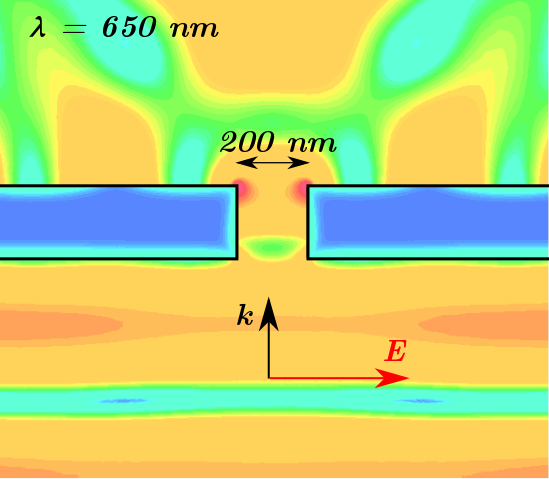
\includegraphics[scale=.3]{E_squared_final.png}
        \caption{Subwavelength Transmission through a Silver slit}
      \end{figure}
      \end{column}%
    \end{columns}
  \end{frame}
% ------------------------------------------------------------
% ------------------------------------------------------------
% ------------------------------------------------------------
% ------------------------------------------------------------
% ------------------------------------------------------------
% ------------------------------------------------------------
% ------------------------------------------------------------
% ------------------------------------------------------------
\begin{frame}
  \frametitle{Background}
  \framesubtitle{Optical Nanoantennas}

  \begin{columns} % align columns
    \begin{column}{.45\textwidth}
      % \begin{minipage}[T][.1\textheight][c]{\linewidth}
      \vspace*{-1cm}
      \begin{itemize}
        \item Convert Localized near-field to efficient far-field radiation
        \item Low Q-factor
        \item Extremely small size
        \item \color{red}{High Purcell Factor}
      \end{itemize}
      \begin{equation} \nonumber
        \mathrm{P}  = \frac{\mathrm{Q}}{\mathrm{V}}
      \end{equation}
      \begin{itemize}
        \item Directive radiation
      \end{itemize}
      % \end{minipage}
      %
    \end{column}
    %
    \begin{column}{.55\textwidth}
      \vspace*{-1cm}
      % Use this to preserve fonts from Inkspace
      \begin{figure}
        \hspace*{-1cm}
        \def\svgwidth{\linewidth}
        \input{figures/curto.pdf_tex}
        \caption{Optical resonant cavities for electric field enhancement}
      \end{figure}
      \end{column}%
    \end{columns}
  \end{frame}
% ------------------------------------------------------------
% ------------------------------------------------------------
% ------------------------------------------------------------
% ------------------------------------------------------------
% ------------------------------------------------------------
% ------------------------------------------------------------
% ------------------------------------------------------------
% ------------------------------------------------------------
\begin{frame}
  \frametitle{Background}
  \framesubtitle{Optical Nanoantennas (contd.)}

  \begin{columns} % align columns
    \begin{column}{.45\textwidth}
      \begin{minipage}[T][.1\textheight][c]{\linewidth}
        \begin{itemize}
          \item Scaled-down microwave designs
          \begin{itemize}
            \item[-] Directivity: Yagi-Uda antenna
            \item[-] Broadband: Bowtie antenna
          \end{itemize}
        \end{itemize}
        \begin{figure}
          \includegraphics[scale=.03]{bowtie_field_map.png}
          % \caption{Subwavelength Transmission through a Silver slit}
        \end{figure}
      \end{minipage}
    \end{column}
    %
    \begin{column}{.55\textwidth}
      % Use this to preserve fonts from Inkspace
      \hspace*{-1cm}
      \vspace*{-1cm}
      \begin{figure}
        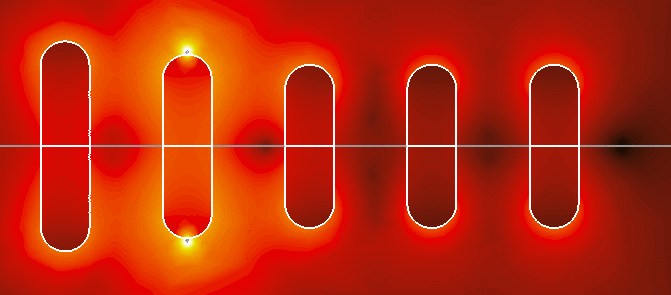
\includegraphics[scale=.04]{yagi_fields.png}
        % \caption{Subwavelength Transmission through a Silver slit}
      \end{figure}
      \hspace*{-1cm}
      \vspace*{-1.2cm}
      \begin{figure}

        \includegraphics[scale=.3]{yagi_patterna.png}
        % \caption{Subwavelength Transmission through a Silver slit}
      \end{figure}
      \end{column}%
    \end{columns}
  \end{frame}
  % ------------------------------------------------------------
  % ------------------------------------------------------------
  % ------------------------------------------------------------
  % ------------------------------------------------------------
  % ------------------------------------------------------------
  % ------------------------------------------------------------
  % ------------------------------------------------------------
  \begin{frame}
    \frametitle{Background}
    \framesubtitle{Optical Nanoantennas}
    \begin{columns}[T] % align columns
      \begin{column}{.5\textwidth}
        \begin{itemize}
          \item Metal-dielectric Interface
        \end{itemize}
        \begin{equation} \nonumber
          k_{sp}=\frac{\O}{c}\sqrt {\dfrac {\E_{1}\E_{2}(\O)} {\E_{1} + \E_{2}(\O)}}
          \label{eq:dis_spp}
        \end{equation}
        \begin{itemize}
          \item Accurate material description using Drude-critical points
        \end{itemize}
        \begin{equation} \nonumber
          \E_2(\O) = \E_{\inf} - \frac{\O_{d}^{2}}{\O^2 + j\gamma \O} + \sum \limits_{i = 1}^N G_i(\O)
          \label{eq:eps_drude_cp}
        \end{equation}
        \begin{equation} \nonumber
          G_i(\O) = C_i \left[ \frac{e^{j \phi_i}}{\O_i - \O - j \Gamma_i} + \frac{e^{-j \phi_i}}{\O_i + \O + j \Gamma_i} \right]
          \label{eq:CP_terms}
        \end{equation}
      \end{column}
      \begin{column}[T]{.5\textwidth}
        \begin{figure}
          \vspace*{-2cm}
          \includestandalone[width=.75\linewidth]{figures/ep_gold}
          \label{fig:ep_gold}
          \caption{Dispesion curve for Gold-air SPPs}
        \end{figure}
        \begin{figure}
          \vspace*{-1cm}
          \includestandalone[width=.75\linewidth]{figures/disp_gold}
          \label{fig:disp_gold}
        \end{figure}
      \end{column}
    \end{columns}
  \end{frame}
% ------------------------------------------------------------
% ------------------------------------------------------------
% ------------------------------------------------------------
% ------------------------------------------------------------
% ------------------------------------------------------------
% ------------------------------------------------------------
% ------------------------------------------------------------
% ------------------------------------------------------------
\begin{frame}
  \frametitle{Background}
  \framesubtitle{Two-dimensional Electon Gas (2DEG)}

  \begin{columns} % align columns
    \begin{column}{.5\textwidth}
      \begin{minipage}[T][.1\textheight][c]{\linewidth}
        \begin{itemize}
          \item Semiconductor Heterostructure Interface
          \item High concentration of free electrons
          \item \textbf{Two-dimensional Surface waves}
          \item Formation of Quantum Well
          \begin{itemize}
            \item[]{Two-dimensional confinement of electrons}
          \end{itemize}
        \end{itemize}
      \end{minipage}
      %
    \end{column}
    %
    \begin{column}{.5\textwidth}
      % Use this to preserve fonts from Inkspace
      \begin{figure}
        \def\svgwidth{\linewidth}
        \input{figures/hemt.pdf_tex}
        \caption{Typical GaAs/AlGaAs HEMT}
      \end{figure}
      \end{column}%
    \end{columns}
  \end{frame}
% ------------------------------------------------------------
% ------------------------------------------------------------
% ------------------------------------------------------------
% ------------------------------------------------------------
% ------------------------------------------------------------
% ------------------------------------------------------------
% ------------------------------------------------------------
% ------------------------------------------------------------
\begin{frame}
  \frametitle{Background}
  \framesubtitle{2DEG (contd.)}

  \begin{columns} % align columns
    \begin{column}{.5\textwidth}
      \begin{minipage}[T][.1\textheight][c]{\linewidth}
        \begin{itemize}
          \item Plasma waves in 2DEG
          \item Dyakonov-Shur instability
          \begin{itemize}
            \item[-]{Voltage bias at source and drain terminals}
            \item[-]{Plasma resonance}
            \item[-]{Emission of terahertz radiation}
            \item[-]{External radiation detection}
          \end{itemize}
          \item \emph{Electronic Flute}
          \item Tunable resonance with gate voltage
          \item Shallow water waves
          \begin{itemize}
            \item[-]{\color{red}Surface waves}
          \end{itemize}
        \end{itemize}
      \end{minipage}
      %
    \end{column}
    %
    \begin{column}{.5\textwidth}
      % Use this to preserve fonts from Inkspace
      \begin{figure}
        \def\svgwidth{\linewidth}
        \input{figures/flute_2deg.pdf_tex}
        % \caption{Typical GaAs/AlGaAs HEMT}
      \end{figure}
      \begin{equation} \nonumber
        \begin{split}
          \lambda &= \frac{c}{f} \\
          & \Longrightarrow  300 \u \mathrm{m}
        \end{split}
        \label{eq:disp_TE_two}
      \end{equation}
      \end{column}%
    \end{columns}
  \end{frame}
% ------------------------------------------------------------
% ------------------------------------------------------------
% ------------------------------------------------------------
% ------------------------------------------------------------
% ------------------------------------------------------------
% ------------------------------------------------------------
% -------------------THEORY-----------------------------------
% ------------------------------------------------------------
% ------------------------------------------------------------
% ------------------------------------------------------------
% ------------------------------------------------------------
% ------------------------------------------------------------
% ------------------------------------------------------------
% ------------------------------------------------------------
% ------------------------------------------------------------
% ------------------------------------------------------------
% Beginning of the actual content
\section{Theory}
\begin{frame}
  \frametitle{Theory}
  \framesubtitle{2DEG formation}
  \begin{columns} % align columns
    \begin{column}{.5\textwidth}
      \begin{minipage}[T][.1\textheight][c]{\linewidth}
        \begin{itemize}
          \item Interface of two slightly different semiconductors/insulators
          \item High electron concentration ($\sim 10^{12}-10^{14} cm^{-2}$)
          \item Triangular quantum well
          \begin{itemize}
            \item[]{Entrapment of electrons in transverse direction}
            \item[]{Free lateral movement}
          \end{itemize}
        \end{itemize}
      \end{minipage}
      %
    \end{column}
    %
    \begin{column}{.5\textwidth}
      % Use this to preserve fonts from Inkspace
      \begin{figure}
        \vspace*{-1cm}
        \def\svgwidth{\linewidth}
        \input{figures/2deg_bandgap.pdf_tex}
        \caption{Band diagram of a GaAs/AlGaAs heterostructure}
      \end{figure}
      \begin{itemize}
        \item[]{\makebox[.5cm][l]{$E_c$} - Conduction band edge}
        \item[]{\makebox[.5cm][l]{$E_f$} - Fermi level}
      \end{itemize}
      \end{column}%
    \end{columns}
  \end{frame}
% ------------------------------------------------------------
% ------------------------------------------------------------
% ------------------------------------------------------------
% ------------------------------------------------------------
% ------------------------------------------------------------
% ------------------------------------------------------------
% ------------------------------------------------------------
\begin{frame}

  \frametitle{Theory}
  \framesubtitle{2DEG Dispersion Relation}
  \vspace*{-.5cm}
  \begin{columns} % align columns
    \begin{column}[T]{.5\textwidth}
      \begin{itemize}
        \item TE mode
      \end{itemize}
      \begin{equation} \nonumber
        k_{z1} + k_{z2} = \O \sigma_s(\O)
        \label{eq:disp_TE_two}
      \end{equation}
      \begin{itemize}
        \item[] No real solutions for an isotropic environment
      \end{itemize}
      \begin{itemize}
        \item TM mode
      \end{itemize}
      \begin{equation} \nonumber
        \tcbhighmath[drop fuzzy shadow]{\frac{\E_1(\O)}{k_{z1}} + \frac{\E_2(\O)}{k_{z2}} = -\frac{\sigma_s(\O)}{\O}}
        \label{eq:disp_TM_two}
      \end{equation}
      \begin{itemize}
        \item[] Real solution(s). Surface waves exist.
      \end{itemize}
    \end{column}
    %
    \begin{column}[T]{.5\textwidth}
      \begin{equation} \nonumber
        \begin{split}
          k_{zi} = \sqrt{\left(\frac{\O}{c}\right)^2 \E_i(\O) -  k_x^2}
        \end{split}
        \label{eq:kz}
      \end{equation}
      % Use this to preserve fonts from Inkspace
      \begin{figure}
        \def\svgwidth{\linewidth}
        \input{figures/2deg.pdf_tex}
        \caption{2DEG at a semiconductor heterojunction}
      \end{figure}
      \end{column}%
    \end{columns}
  \end{frame}
% ------------------------------------------------------------
% ------------------------------------------------------------
% ------------------------------------------------------------
% ------------------------------------------------------------
% ------------------------------------------------------------
% ------------------------------------------------------------
% ------------------------------------------------------------
\begin{frame}
  \frametitle{Theory}
  \framesubtitle{Material Description}
  \begin{columns}[T] % align columns
    \begin{column}{.5\textwidth}
      \begin{itemize}
        \item Complex valued
        \item Drude-Lorentz oscillator model
      \end{itemize}
      \begin{equation} \nonumber
        \E(\O) = \E^{\inf} + \prod_i\frac{\O_{li}^2 - \O^2 - j\gamma_{li} \O}{\O_{ti}^2 - \O^2 - j\gamma_{ti} \O}
        \label{eq:eps}
      \end{equation}
      \begin{itemize}
        \item[]{\makebox[.3cm][l]{$\E^{\inf}$} - High-frequency limit}
        \item[]{\makebox[.3cm][l]{$\O_{ti}$} - TO phonon frequencies}
        \item[]{\makebox[.3cm][l]{$\O_{li}$} - LO phonon frequencies}
        \item[]{\makebox[.3cm][l]{$\gamma$} - Damping constants}
      \end{itemize}
    \end{column}
    \begin{column}[T]{.5\textwidth}
      % \begin{figure}
      %   \vspace*{-2cm}
      %   \subfloat[]{\includestandalone[width=.65\linewidth,keepaspectratio]{figures/epsilon_gaas}
      %   \label{fig:eps_Ga}}
      %   \vspace*{0cm}
      %   \subfloat[Dispersion curve]{\includestandalone[width=.65\linewidth,keepaspectratio]{figures/dispersion_gaas}
      %   \label{fig:eps_Sto}}
      %   % \caption{Dielectric Functions of the materials in bulk form. Solid line: real part, dashed line: imaginary part}
      %   % \label{fig:eps}
      % \end{figure}
      \end{column}%
    \end{columns}
  \end{frame}
% ------------------------------------------------------------
% ------------------------------------------------------------
% ------------------------------------------------------------
% ------------------------------------------------------------
% ------------------------------------------------------------
% ------------------------------------------------------------
% ------------------------------------------------------------
\begin{frame}
\frametitle{Theory}
\framesubtitle{Thin Sheet Simulation}
\begin{columns}[T] % align columns
\begin{column}{.5\textwidth}
  \begin{itemize}
    \item{Volume Integral formulation}
  \end{itemize}
  \begin{equation} \nonumber
    \begin{split}
      \v A &= \frac{\u}{4 \pi} \int\limits_{V} \v J_v(\v r')  \frac{ e^{-j k_1 |\v r - \v r'|}}{|\v r - \v r'|} \diff{v'} \\
      \v E_1^{scat} &= -\frac{j \O}{k_1^2} \left( k_1^2 + \del \del \cdot \right) \v A \\
      \v J_v &= \frac{-j k_1}{Z_0}(\E_2 - 1)\v E_2
    \end{split}
    \label{eq:E1sc}
  \end{equation}
  \begin{itemize}
    \item{Surface current $J_s$ approximated from $J_v$}
  \end{itemize}
\end{column}
\begin{column}[T]{.5\textwidth}
  \vspace*{-2cm}
  \begin{itemize}
    \item{Impedance (Leontovich) Boundary Conditions}
  \end{itemize}
  \begin{equation} \nonumber
    \v E_{tan} = \eta Z_0 \hat{\v n} \times \v H
    \label{eq:eps}
  \end{equation}
  \begin{equation} \nonumber
    \begin{split}
      E^i &= \eta Z_0 J_s(x') \\
      & + \frac{\O \u}{4}  \int\limits_{l} J_s(x')  H_0^{(2)}(k_2 |x - x'|) \diff{x'}
    \end{split}
    \label{eq:eps}
  \end{equation}
  % Use this to preserve fonts from Inkspace
  \begin{figure}
    \def\svgwidth{.75\linewidth}
    \input{figures/seniors.pdf_tex}
    \caption{Dielectric Slab geometry}
  \end{figure}
  \end{column}%
\end{columns}
\end{frame}
% ------------------------------------------------------------
% ------------------------------------------------------------
% ------------------------------------------------------------
% ------------------------------------------------------------
% ------------------------------------------------------------
% ------------------------------------------------------------
% ------------------------------------------------------------
% ------------------------------------------------------------
% ------------------------------------------------------------
% ------------------------------------------------------------
% ------------------------------------------------------------
% ------------------------------------------------------------
% ------------------------------------------------------------
% ------------------------------------------------------------
\section{Results}

\begin{frame}
  \frametitle{Proposed Scheme}
  \framesubtitle{Surface Integral Equation}

  \begin{itemize}
    \item{Surface Equivalence Theorem}
  \end{itemize}
  \begin{figure}
    \centering
    \def\svgwidth{1\linewidth}
    \input{figures/equivalence.pdf_tex}
    \caption{(a). Actual and its equivalent models for the (b) external and, (c) Internal region }
  \end{figure}
\end{frame}
% ------------------------------------------------------------
% ------------------------------------------------------------
% ------------------------------------------------------------
% ------------------------------------------------------------
% ------------------------------------------------------------
% ------------------------------------------------------------
% ------------------------------------------------------------
\begin{frame}
\frametitle{Proposed Scheme}
\framesubtitle{Surface Integral Equation}
\vspace*{-.4cm}
\begin{itemize}
  \item{Exterior Region}
\end{itemize}
\begin{equation} \nonumber
  \begin{split}
    \v E_1 &= \v E_i + \v E_1^{scat} \\
    &=  -\frac{\O}{4 k_1^2} \left( k_1^2 + \del \del \cdot \right) \int\limits_{C} \v J_s(\v p') H_0^{(2)}(k_1 |\v \p - \v \p'|) \diff{l'} \\
    &- \frac{1}{4 \E j} \del \x \int\limits_{l} \v M_s(\v \p') H_0^{(2)}(k_1 |\v \p - \v \p'|) \diff{l'} + \v E_i
  \end{split}
  \label{eq:E1sc}
\end{equation}
\begin{equation} \nonumber
  \begin{split}
    \v H_1 &= \v H_i + \v H_1^{scat} \\
    &= \frac{1}{4 j} \del \x \int\limits_{l} \v J_s(\v \p') H_0^{(2)}(k_1 |\v \p - \v \p'|) \diff{l'} \\
    &-\frac{\O}{4 k_1^2} \left( k_1^2 + \del \del \cdot \right) \int\limits_{l} \v M_s(\v \p') H_0^{(2)}(k_1 |\v \p - \v \p'|) \diff{l'} + \v H_i
  \end{split}
  \label{eq:H1sc}
\end{equation}
\end{frame}
% ------------------------------------------------------------
% ------------------------------------------------------------
% ------------------------------------------------------------
% ------------------------------------------------------------
% ------------------------------------------------------------
% ------------------------------------------------------------
% ------------------------------------------------------------
\begin{frame}
\frametitle{Proposed Scheme}
\framesubtitle{Surface Integral Equation}
\vspace*{-.4cm}
\begin{itemize}
  \item{Interior Region}
\end{itemize}
\begin{equation} \nonumber
  \begin{split}
    \v E_2 &= \v E_2^{scat} \\
    &=  -\frac{\O}{4 k_2^2} \left( k_2^2 + \del \del \cdot \right) \int\limits_{C} \left(-\v J_s(\v p')\right) H_0^{(2)}(k_2 |\v \p - \v \p'|) \diff{l'} \\
    &- \frac{1}{4 j} \del \x \int\limits_{l} \left(-\v M_s(\v \p')\right) H_0^{(2)}(k_2 |\v \p - \v \p'|) \diff{l'}
  \end{split}
  \label{eq:E1sc}
\end{equation}
\begin{equation} \nonumber
  \begin{split}
    \v H_2 &= \v H_1^{scat} \\
    &= \frac{1}{4 j} \del \x \int\limits_{l} \left(-\v J_s(\v \p')\right) H_0^{(2)}(k_2 |\v \p - \v \p'|) \diff{l'} \\
    &-\frac{\O}{4 k_2^2} \left( k_2^2 + \del \del \cdot \right) \int\limits_{l} \left(-\v M_s(\v \p')\right) H_0^{(2)}(k_2 |\v \p - \v \p'|) \diff{l'}
  \end{split}
  \label{eq:H1sc}
\end{equation}
\end{frame}
% ------------------------------------------------------------
% ------------------------------------------------------------
% ------------------------------------------------------------
% ------------------------------------------------------------
% ------------------------------------------------------------
% ------------------------------------------------------------
% ------------------------------------------------------------
\begin{frame}
\frametitle{Proposed Scheme}
\framesubtitle{Thin Flat Sheet $TM_z$}
\begin{equation} \nonumber
  \hat{\v n} \x (\v E_1 - \v E_2) = \v 0
  \label{eq:E1bc}
\end{equation}
\begin{align} \nonumber
  E_i ={}& \frac{\O}{4} \int\limits_L J_z(x') \left[ H_0^{(2)}(k_1 | x -  x'|) + H_0^{(2)}(k_2 |x - x'|)\right] \diff{x'}  \notag
  \label{eq:scalarE}
\end{align}
\begin{equation} \nonumber
  \hat{\v n} \x (\v H_1 - \v H_2) = \v 0
  \label{eq:E1bc}
\end{equation}
\begin{align} \nonumber
  H_i^{tan} &= \frac{-j \O}{2} \int\limits_L M_x(x') \left[ \E_1 H_0^{(2)}(k_1 |x - x'|) + \E_1 H_2^{(2)}(k_1 |x - x'|) \right. \notag\\
  & \left. + \E_2 H_0^{(2)}(k_2 |x - x'|) + \E_2 H_2^{(2)}(k_2 |x - x'|)\right] \diff{x'} \notag
  \label{eq:scalarH}
\end{align}
\end{frame}
% ------------------------------------------------------------
% ------------------------------------------------------------
% ------------------------------------------------------------
% ------------------------------------------------------------
% ------------------------------------------------------------
% ------------------------------------------------------------
% ------------------------------------------------------------
\begin{frame}
  \frametitle{Proposed Scheme}
  \framesubtitle{Method of moments}
  \begin{itemize}
    \item {Integral equations to system of linear equations}
  \end{itemize}
  \[
  \begin{bmatrix}
    Z_{mn}   & 0 \\
    0        & Y_{mn}
  \end{bmatrix}
  \begin{bmatrix}
    J_n \\
    M_n
  \end{bmatrix}
  =
  \begin{bmatrix}
    E_m^i \\
    H_m^i
  \end{bmatrix}
  \]
  \begin{itemize}
    \item {Pulse basis functions and Point matching used}
    \item {Far-field}
  \end{itemize}
  \begin{equation} \nonumber
  RCS({\phi}) \simeq \int \limits_{0}^{L} \left[J_z(x')\eta_1 + M_x(x')\sin(\phi_i)\right] e^{j k_1 x' \cos(\phi_i)} \mathrm{d}x'
  \label{eq:far-field}
\end{equation}
\end{frame}
% ------------------------------------------------------------
% ------------------------------------------------------------
% ------------------------------------------------------------
% ------------------------------------------------------------
% ------------------------------------------------------------
% ------------------------------------------------------------
% ------------------------------------------------------------

\begin{frame}
\frametitle{Results}
\framesubtitle{Thin Sheet Simulation ($TM_z$)}
\begin{columns}[T] % align columns
  \begin{column}{.5\textwidth}
    \begin{itemize}
      \item[-]{$TM_z$ polarization}
      \item[-]{Dielectric Rod of length 2.5 $\lambda$}
      \item[-]{$\E = 4$, $\u = 1$}
    \end{itemize}
    \begin{figure}[h]
      \normalsize
      \centering
      \includestandalone[width=\textwidth]{figures/tm_plate}
      \caption{Thin sheet under $\mathrm{TM_z}$ polarized plane wave incidence}
      \label{fig:tm_plate}
    \end{figure}
  \end{column}
  \begin{column}[T]{.5\textwidth}
    \begin{figure}
      \vspace*{-2cm}
      \includestandalone[width=\linewidth,keepaspectratio]{figures/richmond_tm2}
      \caption{Radar Cross-section}
      \label{fig:TM_rcs}
    \end{figure}
    \begin{itemize}
      \item[-]{Thickness of $.05 \lambda$ assumed in Volume Integral equation model}
    \end{itemize}
    \end{column}%
  \end{columns}
\end{frame}
% ------------------------------------------------------------
% ------------------------------------------------------------
% ------------------------------------------------------------
% ------------------------------------------------------------
% ------------------------------------------------------------
% ------------------------------------------------------------
% ------------------------------------------------------------
\begin{frame}
  \frametitle{Results}
  \framesubtitle{Thin Sheet Simulation ($TE_z$)}
  \begin{columns}[T] % align columns
    \begin{column}{.5\textwidth}
      \begin{itemize}
        \item[-]{$TE_z$ polarization}
        \item[-]{Dielectric Rod of length 2.5 $\lambda$}
        \item[-]{$\E = 4$, $\u = 1$}
      \end{itemize}
      \begin{figure}[h]
        \normalsize
        \centering
        \includestandalone[width=\textwidth]{figures/te_plate}
        \caption{Thin sheet under $\mathrm{TE_z}$ polarized plane wave incidence}
        \label{fig:te_plate}
      \end{figure}
    \end{column}
    \begin{column}[T]{.5\textwidth}
      \begin{figure}
        \vspace*{-2cm}
        \includestandalone[width=\linewidth,keepaspectratio]{figures/richmond_te1}
        % \caption{Radar Cross-section}
        \label{fig:TE_rcs}
      \end{figure}
      \begin{itemize}
        \item[-]{Thickness of $.05 \lambda$ assumed in Volume Integral equation model}
      \end{itemize}
      \end{column}%
  \end{columns}
\end{frame}
% ------------------------------------------------------------
% ------------------------------------------------------------
% ------------------------------------------------------------
% ------------------------------------------------------------
% ------------------------------------------------------------
% ------------------------------------------------------------
% ------------------------------------------------------------
\begin{frame}
  \frametitle{Results}
  \framesubtitle{Thin Sheet Simulation ($TE_z$)}
  \begin{columns}[T] % align columns
    \begin{column}{.5\textwidth}
      \begin{itemize}
        \item[-]{$TE_z$ polarization}
        \item[-]{Dielectric Rod of length 2 $\lambda$}
        \item[-]{$\E = 4$, $\u = 1$}
      \end{itemize}
      \begin{figure}[h]
        \normalsize
        \centering
        \includestandalone[width=\textwidth]{figures/te_plate}
        \caption{Thin sheet under $\mathrm{TE_z}$ polarized plane wave incidence}
        \label{fig:te_plate}
      \end{figure}
    \end{column}
    \begin{column}[T]{.5\textwidth}
      \begin{figure}
        \vspace*{-2cm}
        \includestandalone[width=\linewidth,keepaspectratio]{figures/farfield_2}
        % \caption{Radar Cross-section}
        \label{fig:TE_rcs}
      \end{figure}
      \begin{itemize}
        \item[-]{Thickness of $.628/k_1$ assumed in resistive model}
      \end{itemize}
      \end{column}%
  \end{columns}
\end{frame}
% ------------------------------------------------------------
% ------------------------------------------------------------
% ------------------------------------------------------------
% ------------------------------------------------------------
% ------------------------------------------------------------
% ------------------------------------------------------------
% ------------------------------------------------------------
\section{Future Work}
% ------------------------------------------------------------
% ------------------------------------------------------------
% ------------------------------------------------------------
% ------------------------------------------------------------
% ------------------------------------------------------------
% ------------------------------------------------------------
\begin{frame}
  \frametitle{Field Computation}
  \framesubtitle{Integral Equations}
  \begin{columns} % align columns
    \begin{column}[T]{.5\textwidth}
      \begin{itemize}
        \item Difficulty in simulation of thin objects
        \item Dense mesh
        \item Computationally expensive
        \item No guarantee of correct solution
      \end{itemize}
    \end{column}
    \begin{column}[T]{.5\textwidth}
      \begin{figure}[!t]
         \noindent
         \includegraphics[width=1\textwidth]{figures/mesh.png}
         \caption{Typical mesh for a dielectric plate of thickness $.05 \u m$}
         \label{fig:mesh}
      \end{figure}
      \end{column}%
    \end{columns}
  \end{frame}
  % ------------------------------------------------------------
  % ------------------------------------------------------------
  % ------------------------------------------------------------
  % ------------------------------------------------------------
  % ------------------------------------------------------------
  % ------------------------------------------------------------
  % ------------------------------------------------------------
  % ------------------------------------------------------------
\begin{frame}
  \frametitle{Future Work}
  \framesubtitle{Use of oxide-based 2DEGs}
  \begin{columns}[T] % align columns
    \begin{column}{.5\textwidth}
      \begin{itemize}
        \item Perovskite oxides
        \item Higher electron concentration $( \sim 10^{14} cm^{-2})$
        \item Higher wave confinement
      \end{itemize}
    \end{column}
    \begin{column}[T]{.5\textwidth}
      % \begin{figure}
      %   \vspace*{-2cm}
      %   \subfloat{\includestandalone[width=.65\linewidth,keepaspectratio]{figures/epsilon_sto}
      %   \label{fig:eps_Ga}}
      %   \vspace*{0cm}
      %   \subfloat[Dispersion curve]{\includestandalone[width=.65\linewidth,keepaspectratio]{figures/dispersion_sto}
      %   \label{fig:eps_Sto}}
      %   % \caption{Dielectric Functions of the materials in bulk form. Solid line: real part, dashed line: imaginary part}
      %   % \label{fig:eps}
      % \end{figure}
      \end{column}%
    \end{columns}
  \end{frame}
  % ------------------------------------------------------------
  % ------------------------------------------------------------
  % ------------------------------------------------------------
  % ------------------------------------------------------------
  % ------------------------------------------------------------
  % ------------------------------------------------------------
  % ------------------------------------------------------------
\begin{frame}
  \frametitle{Nanoscale Imaging scheme}
  \framesubtitle{Remove metal gate}
      % Discuss loss in the scheme
      \begin{figure}[t!]
        \subfloat[]{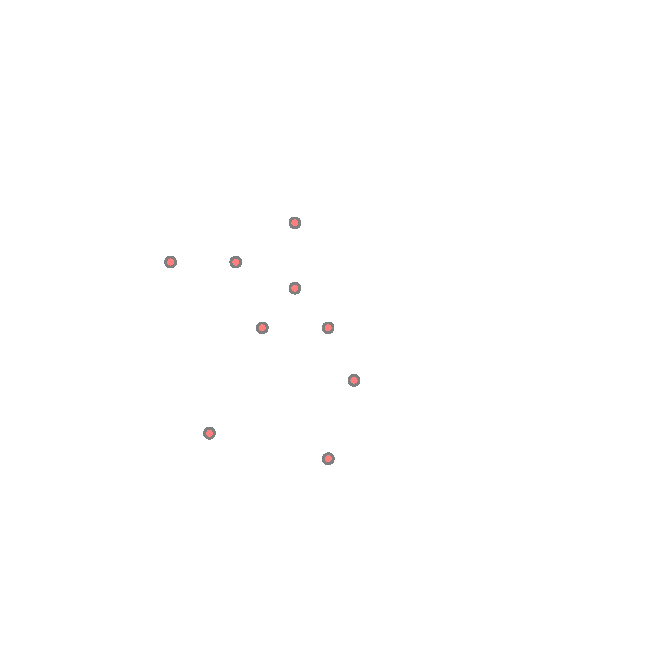
\includegraphics[height = 1.9in]{test_sample.tex}
        \label{fig:test}} \hfil
        \subfloat[]{\includegraphics[height = 1.9in]{plsim_153.tex}
        \label{fig:sim_lo}} \hfil
        \subfloat[]{\includegraphics[height = 1.9in]{plsim_75.tikz}
        \label{fig:sim_hi}}
        \caption{(a) Sample distribution. Simulation of the reconstructed sample image at: (b) $\Re k_{\p} = 39.5$ (c) $\Re k_{\p} = 80$}
        \label{fig:simulation}
      \end{figure}
\end{frame}
% ------------------------------------------------------------
% ------------------------------------------------------------
% ------------------------------------------------------------
% ------------------------------------------------------------
% ------------------------------------------------------------
% ------------------------------------------------------------
% ------------------------------------------------------------
\begin{frame}
\frametitle{Future Work}
\framesubtitle{3D Computation of fields}
\begin{columns}[T] % align columns
  \begin{column}{.5\textwidth}
    \begin{itemize}
      \item Incorporate lateral effects
      \item Model 2DEG as a plate
      \item Investigate effects of finite thickness
    \end{itemize}
  \end{column}
  \begin{column}[T]{.5\textwidth}
    \begin{figure}
      \centering
      \def\svgwidth{1\linewidth}
      \input{figures/2deg_3d.pdf_tex}
      % \caption{(a). Actual and its equivalent models for the (b) external and, (c) Internal region }
    \end{figure}
  \end{column}%
\end{columns}
\end{frame}
% ------------------------------------------------------------
% ------------------------------------------------------------
% ------------------------------------------------------------
% ------------------------------------------------------------
% ------------------------------------------------------------
% ------------------------------------------------------------
% ------------------------------------------------------------
\begin{frame}
\frametitle{Future Recommendations}
\framesubtitle{3D Computation of fields}
\begin{columns}[T] % align columns
  \begin{column}{.5\textwidth}
    \begin{itemize}
      \item Modeling of a 2DEG by surface conductivity tensor
      \item Going beyond III-V materials (perovskites, dichalcogenides)
      \item
    \end{itemize}
  \end{column}
  \begin{column}[T]{.5\textwidth}
    \begin{figure}
      \vspace*{-2cm}
      \subfloat{\includestandalone[width=.65\linewidth,keepaspectratio]{figures/tm_tail}
      \label{fig:eps_Ga}}
      \vspace*{0cm}
      \subfloat{\includestandalone[width=.65\linewidth,keepaspectratio]{figures/te_tail}
      \label{fig:eps_Sto}}
      \caption{Sommerfeld integrals for Green function for a horizontal dipole. (a) Horizontal (TE) (b) Vertical Component (TM)}
      % \label{fig:eps}
    \end{figure}
    \end{column}%
\end{columns}
\end{frame}
% ------------------------------------------------------------
% ------------------------------------------------------------
% ------------------------------------------------------------
% ------------------------------------------------------------
% ------------------------------------------------------------
% ------------------------------------------------------------
% ------------------------------------------------------------
\section{Conclusion}
\begin{frame}
\frametitle{Summary}
\framesubtitle{Two-dimensional plasmonic devices}
    \begin{itemize}
      \item Subwavelength wave phenomena at optical and terahertz frequencies
      \item Realization of terahertz sources and sensors
      \item 2D nature of waves permits subwavelength confinement
      \item Plasmonic activity
      \item Nanoscale imaging using terahertz plasma waves
    \end{itemize}
\end{frame}
% ------------------------------------------------------------
% ------------------------------------------------------------
% ------------------------------------------------------------
% ------------------------------------------------------------
% ------------------------------------------------------------
% ------------------------------------------------------------
% ------------------------------------------------------------
\begin{frame}
\frametitle{Acknowledgements}
\framesubtitle{Sponsorship}
    \begin{itemize}
      \item The Fulbright Program
    \end{itemize}
    \begin{figure}
      \centering
      \def\svgwidth{.4\linewidth}
      \input{figures/fulbright.pdf_tex}
      % \caption{(a). Actual and its equivalent models for the (b) external and, (c) Internal region }
    \end{figure}
\end{frame}
% ------------------------------------------------------------
% ------------------------------------------------------------
% ------------------------------------------------------------
% ------------------------------------------------------------
% ------------------------------------------------------------
% ------------------------------------------------------------
% ------------------------------------------------------------
\begin{frame}[plain,c]
  \begin{center}
    \Huge Thank you!
  \end{center}
\end{frame}
% ------------------------------------------------------------
% ------------------------------------------------------------
% ------------------------------------------------------------
% ------------------------------------------------------------
% ------------------------------------------------------------
% ------------------------------------------------------------
% ------------------------------------------------------------
\begin{frame}[plain,c]
  \begin{center}
    \Huge Questions?
  \end{center}
\end{frame}
  \end{document}
